\section{Bayesian Decision Theory and Probability Estimation}
\label{sec:bayes}

Every image analysis system eventually has to commit to a decision: this pixel
is road, this window contains a pedestrian, this lesion should be referred to a
doctor. The evidence behind such decisions is never certain. Noise corrupts the
measurements, classes overlap in feature space, and the same appearance can be
produced by different causes. Probability theory is the language that turns this
uncertainty into something we can compute with, and Bayesian decision theory
says how to act optimally once the uncertainty has been quantified.

The chain of reasoning in this section runs in three steps. First, a decision
is made by comparing \emph{posterior} probabilities $P(\omega\mid x)$ of the
possible classes $\omega$ given an observation $x$, possibly weighted by the
cost of each mistake. Second, the posterior is assembled from a
\emph{likelihood} $p(x\mid\omega)$ and a \emph{prior} $P(\omega)$ with Bayes'
theorem, exactly as in the scene-inference formula of the introduction. Third,
the likelihood is almost never given and has to be \emph{estimated} from
training data, either without assumptions about its shape (histograms, Parzen
windows, nearest neighbors) or by fitting the parameters of an assumed model
(maximum likelihood and Bayesian estimation). The section closes with Markov
random fields, where the prior is not a single number per class but a model of
how neighboring pixels depend on each other, which lets prior knowledge repair
noisy image data.

\subsection{Probability Basics}

A probability assigns to each possible outcome of an experiment a number that
says how much we believe in it. Let $\Omega$ be the \emph{sample space}, the set
of all possible discrete outcomes $\omega$. A function
$P:\Omega\to\mathbb{R}$ is a probability if and only if
\begin{equation}
  P(\omega)\ge 0 \quad\forall\,\omega\in\Omega
  \qquad\text{and}\qquad
  \sum_{\omega\in\Omega} P(\omega) = 1 .
\end{equation}
\noindent
Both conditions together imply $P(\omega)\le 1$. The probability of an event
$E\subseteq\Omega$, a set of outcomes, is the sum over its members,
$P(E) = \sum_{\omega\in E} P(\omega)$.

\paragraph{Densities are not probabilities.}
For a continuous variable such as a grey value or a feature coordinate, a single
exact value has probability zero, because there are infinitely many values
competing for a total mass of one. What exists instead is the
\emph{cumulative distribution function} $F(x) = P(X\le x)$, which increases
monotonically from $\lim_{x\to-\infty}F(x) = 0$ to $\lim_{x\to+\infty}F(x) = 1$.
Its derivative is the \emph{probability density function}
$p(x) = \partial F(x)/\partial x$, with
\begin{equation}
  p(x)\ge 0 \quad\forall\,x,
  \qquad
  \int p(x)\,dx = 1,
  \qquad
  P(x\in E) = \int_{x\in E} p(x)\,dx .
\end{equation}
\noindent
Unlike a probability, a density can be larger than one: a uniform density on the
interval $[0,0.1]$ has the value $10$ everywhere on it. Only its integral over a
region is a probability, and that integral is at most one. Two consequences
appear again and again in exercises. For a Gaussian with $\mu=0$ and $\sigma=1$,
the density at zero is $1/\sqrt{2\pi}\approx 0.40$, but the \emph{probability}
$P(x=0)$ is $0$, because the integral over a single point vanishes. And a
statement like ``$p(x)\le 1$'' is not a property of densities at all.

\paragraph{The Gaussian distribution.}
The most important density is the normal or Gaussian distribution. In $d$
dimensions, with mean vector $\mu$ and covariance matrix $\Sigma$,
\begin{equation}
  p(x) = \frac{1}{(2\pi)^{d/2}\,\lvert\Sigma\rvert^{1/2}}
  \exp\Bigl(-\tfrac{1}{2}(x-\mu)^\top\Sigma^{-1}(x-\mu)\Bigr),
  \label{eq:gauss-nd}
\end{equation}
\noindent
and in one dimension
$p(x) = \frac{1}{\sqrt{2\pi}\,\sigma}\exp\bigl(-\frac{(x-\mu)^2}{2\sigma^2}\bigr)$
with $\mu = E[x] = \int x\,p(x)\,dx$ and
$\sigma^2 = E[(x-\mu)^2] = \int (x-\mu)^2 p(x)\,dx$. It earns its central role
for two reasons. It describes many real phenomena, above all sensor noise,
because by the central limit theorem a sum of many small independent effects is
approximately Gaussian. And it is analytically convenient: parameter estimates
have closed forms, the derivative is simply
$\partial p/\partial x = -\frac{x-\mu}{\sigma^2}\,p(x)$, and the logarithm of the
density is a quadratic function. Among all distributions with a given mean and
variance, the Gaussian has the largest entropy
$H = -\int p(x)\ln p(x)\,dx$, so it is the least committal choice when only
these two moments are known.

\paragraph{Joint, conditional, and marginal probabilities.}
With two random variables $A$ and $B$, the \emph{joint probability}
$P(A=a,B=b)$ is the probability that both take the given values together; it
lives on a two-dimensional table (or, for densities, a two-dimensional surface).
The \emph{conditional probability} $P(A=a\mid B=b)$ is the probability of $a$
once $b$ is known to have happened; it is a one-dimensional slice of the joint,
renormalized so that it sums to one. Three rules connect them:
\begin{align}
  \text{marginalization:}&\quad P(A=a) = \sum_b P(A=a,B=b),
    \qquad p(x) = \int p(x,y)\,dy, \label{eq:marginal}\\
  \text{product rule:}&\quad P(A,B) = P(A\mid B)\,P(B) = P(B\mid A)\,P(A),
    \label{eq:product}\\
  \text{independence:}&\quad P(A\mid B) = P(A)
    \;\Longleftrightarrow\; P(A,B) = P(A)\,P(B). \label{eq:indep}
\end{align}
\noindent
Marginalization removes a variable by summing or integrating it out; for a
density $p(x_1,x_2,x_3)$, both $p(x_2,x_3) = \int p(x)\,dx_1$ and
$p(x_1) = \iint p(x)\,dx_2\,dx_3$ are marginalizations, while rewriting
$p(x) = p(x_1\mid x_2,x_3)\,p(x_2\mid x_3)\,p(x_3)$ is a factorization with the
product rule and $p(x) = p(x_1)p(x_2)p(x_3)$ is an independence assumption.
For independent variables the joint table is the outer product of the
marginals: with $P(a_1) = 0.2$, $P(a_2) = 0.8$ and $P(b_1) = P(b_2) = 0.5$ every
entry is $P(a)\cdot 0.5$, so both rows of the table read $(0.1,\ 0.4)$.

\paragraph{Bayes' theorem.}
The two factorizations in Equation~\eqref{eq:product} describe the same joint
probability, so they must be equal:
$P(A\mid B)\,P(B) = P(B\mid A)\,P(A)$. Dividing by $P(B)$ gives
\begin{equation}
  P(A\mid B) = \frac{P(B\mid A)\,P(A)}{P(B)},
  \qquad
  p(x\mid y) = \frac{p(y\mid x)\,p(x)}{p(y)} .
  \label{eq:bayes}
\end{equation}
\noindent
The theorem inverts a conditional: it computes the probability of a cause given
an effect from the probability of the effect given the cause, which is usually
what we can model. Its four terms have fixed names (Table~\ref{tab:bayes-terms}),
which are asked for directly.

\begin{table}[ht]
  \centering
  \begin{tabular}{@{}llp{7.6cm}@{}}
    \toprule
    Term & Name & Meaning in classification \\
    \midrule
    $P(\omega\mid x)$ & posterior & belief in class $\omega$ after seeing $x$ \\
    $p(x\mid\omega)$ & likelihood & how probable the observation is if the class
      is $\omega$; read as a function of $\omega$ it is the likelihood
      \emph{of the class} \\
    $P(\omega)$ & prior & belief in $\omega$ before any observation \\
    $p(x)$ & evidence & normalizer
      $\sum_j p(x\mid\omega_j)P(\omega_j)$, the same for all classes \\
    \bottomrule
  \end{tabular}
  \caption{The terms of Bayes' theorem $P(\omega\mid x) = p(x\mid\omega)P(\omega)/p(x)$.
  In $P(C=c\mid X=x)$ the quantity is the posterior of the class $C$, not of the
  observation $X$.}
  \label{tab:bayes-terms}
\end{table}

\subsection{Bayesian Decision Theory}

Does a given picture show a tiger? Without looking at it, the only available
knowledge is how common tigers are. If the picture was taken in an Indian jungle
the answer ``tiger'' is more plausible than for a picture from Antarctica. This
is the \emph{prior} $P(\omega)$: knowledge that does not come from the current
observation but from experience, experts, or given information, and that is
often simply assumed uniform. With the two states
$\Omega = \{\omega_1,\omega_2\} = \{\text{tiger},\text{no tiger}\}$ and
$P(\omega_1)+P(\omega_2) = 1$, the best decision \emph{before} observation is
\begin{equation}
  \text{select }\omega_1\text{ if } P(\omega_1) > P(\omega_2),
  \text{ otherwise }\omega_2 .
\end{equation}
\noindent
This rule always gives the same answer, whatever the picture shows. Once the
picture itself or features $x$ extracted from it are available, the decision
should be based on the \emph{posterior} instead: select $\omega_1$ if
$P(\omega_1\mid x) > P(\omega_2\mid x)$. Discriminative methods, such as the
neural networks of Section~\ref{sec:neural-networks} with a softmax output,
model this posterior directly. Generative methods model likelihood and prior and
obtain the posterior with Bayes' theorem.

\paragraph{MAP, ML, and naive Bayes.}
For any number of classes the rule generalizes to picking the class with the
largest posterior. Since the evidence $p(x)$ does not depend on $\omega$, it can
be dropped:
\begin{equation}
  \omega^* = \arg\max_\omega P(\omega\mid x)
  = \arg\max_\omega \frac{p(x\mid\omega)\,P(\omega)}{p(x)}
  = \arg\max_\omega p(x\mid\omega)\,P(\omega).
  \label{eq:map}
\end{equation}
\noindent
This is the \emph{maximum a posteriori} (MAP) estimator. If the prior is
uniform, all classes are equally likely beforehand and $P(\omega)$ drops out as
well, leaving the \emph{maximum likelihood} (ML) estimator
$\omega^* = \arg\max_\omega p(x\mid\omega)$. ML and MAP therefore coincide
exactly when the prior is uniform. When $x$ consists of $F$ features, the
likelihood $p(x\mid\omega)$ is a $F$-dimensional density that is hard to model.
\emph{Naive Bayes} assumes that the features are conditionally independent
given the class,
\begin{equation}
  p(x\mid\omega) = \prod_{i=1}^{F} p(x_i\mid\omega),
\end{equation}
\noindent
so that only $F$ one-dimensional densities per class have to be estimated. The
assumption is rarely true, but the resulting classifier often works well
because the decision only needs the correct \emph{ranking} of the classes.

\paragraph{Working with logarithms.}
Products of many small probabilities underflow numerically, and priors and
likelihoods are easier to compare as sums. Because the logarithm is strictly
increasing, taking it does not change the $\arg\max$. A typical exam situation:
a pixel is foreground ($C=1$) or background ($C=0$), a model supplies
$p(x\mid C=c)$, and foreground covers on average $10\%$ of the image, so
$P(C=1) = 0.1$ and $P(C=0) = 0.9$. The MAP rule labels a pixel as background if
\begin{align}
  0.9\,p(x\mid C=0) > 0.1\,p(x\mid C=1)
  \;&\Longleftrightarrow\;
  9\,p(x\mid C=0) > p(x\mid C=1) \nonumber\\
  &\Longleftrightarrow\;
  \ln p(x\mid C=0) - \ln p(x\mid C=1) > \ln 0.1 - \ln 0.9 .
\end{align}
\noindent
All three forms are the same rule. Comparing only the priors ignores the pixel,
and comparing only the likelihoods is the ML rule, not MAP.

\begin{figure}[!htb]
  \centering
  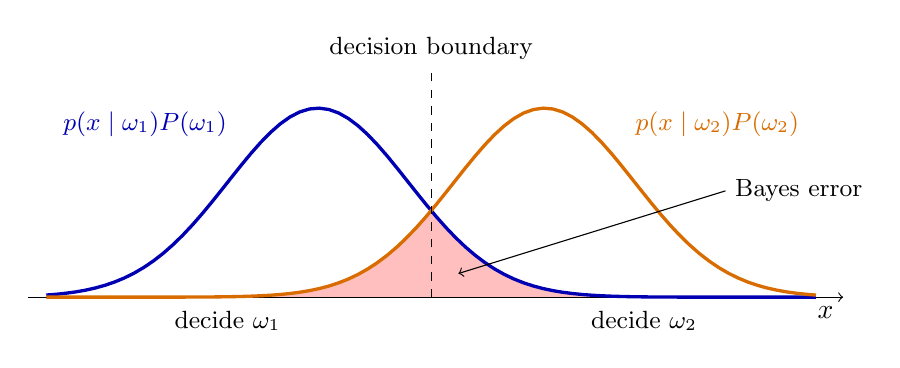
\begin{tikzpicture}[x=1.15cm, y=1cm]
    % weighted likelihoods P(w_i) p(x|w_i), equal priors, sigma = 1
    \fill[red!25, domain=-4:0.25, samples=60]
      (-4,0) -- plot (\x,{2.4*exp(-(\x-1.5)^2/2)}) -- (0.25,0) -- cycle;
    \fill[red!25, domain=0.25:4.5, samples=60]
      (0.25,0) -- plot (\x,{2.4*exp(-(\x+1)^2/2)}) -- (4.5,0) -- cycle;
    \draw[->] (-4.2,0) -- (4.8,0) node[below left] {$x$};
    \draw[very thick, blue!70!black, domain=-4:4.5, samples=80]
      plot (\x,{2.4*exp(-(\x+1)^2/2)});
    \draw[very thick, orange!85!black, domain=-4:4.5, samples=80]
      plot (\x,{2.4*exp(-(\x-1.5)^2/2)});
    \draw[dashed] (0.25,0) -- (0.25,2.9);
    \node[above] at (0.25,2.9) {\small decision boundary};
    \node[blue!70!black, left] at (-1.9,2.2) {\small $p(x\mid\omega_1)P(\omega_1)$};
    \node[orange!85!black, right] at (2.4,2.2) {\small $p(x\mid\omega_2)P(\omega_2)$};
    \node[below] at (-2,-0.05) {\small decide $\omega_1$};
    \node[below] at (2.6,-0.05) {\small decide $\omega_2$};
    \draw[<-] (0.55,0.3) -- (3.5,1.35) node[right] {\small Bayes error};
  \end{tikzpicture}
  \caption{Two classes with equal priors and Gaussian likelihoods. The MAP rule
  switches class where the weighted likelihoods intersect. The shaded area is
  the Bayes error of Equation~\eqref{eq:bayes-error}: the probability mass of
  each class that falls on the wrong side. Increasing $P(\omega_2)$ raises the
  orange curve and moves the boundary toward $\omega_1$.}
  \label{fig:bayes-error}
\end{figure}

\paragraph{Loss and risk.}
Not all mistakes are equally bad. Missing a melanoma is far worse than sending a
harmless lesion for a second inspection. Bayesian decision theory captures this
with a \emph{loss} $\lambda(\alpha_i\mid\omega_j)$, the cost of taking action
$\alpha_i$ when the true state is $\omega_j$. Since the true state is unknown,
each action is judged by its expected loss under the posterior, the
\emph{conditional risk}
\begin{equation}
  R(\alpha_i\mid x) = \sum_{j} \lambda(\alpha_i\mid\omega_j)\,P(\omega_j\mid x),
  \qquad
  \alpha^* = \arg\min_{i} R(\alpha_i\mid x).
  \label{eq:risk}
\end{equation}
\noindent
The posterior says what is likely, the loss says what mistakes cost, and the
decision rule combines both. MAP is the special case of the \emph{0/1 loss}
($\lambda = 0$ for the correct class, $1$ otherwise): then
$R(\alpha_i\mid x) = \sum_{j\ne i}P(\omega_j\mid x) = 1 - P(\omega_i\mid x)$, and
minimizing the risk is maximizing the posterior.

Two worked cases show how to compute with Equation~\eqref{eq:risk}. First, a
diagnostic system with states $\omega_1$ (ill), $\omega_2$ (healthy), actions
$\alpha_1$ (treat) and $\alpha_2$ (do nothing), losses
$\lambda(\alpha_1\mid\omega_1) = 18$, $\lambda(\alpha_1\mid\omega_2) = 2$,
$\lambda(\alpha_2\mid\omega_1) = 57$, $\lambda(\alpha_2\mid\omega_2) = 70$, and
$P(\omega_1\mid x) = 0.75$. The expected risk of treating is
\begin{equation}
  R(\alpha_1\mid x) = 18\cdot 0.75 + 2\cdot 0.25 = 14.00,
\end{equation}
\noindent
and doing nothing would cost $57\cdot 0.75 + 70\cdot 0.25 = 60.25$, so treatment
is chosen. The only care needed is to read the loss table correctly: fix the
action, then sum over the true states weighted by their posteriors. Second, a
binary triage with classes melanoma $M$ and benign $B$, zero cost for correct
decisions, and a false negative five times as costly as a false positive,
$\lambda(\mathrm{FN}) = 5\lambda(\mathrm{FP})$. The risks are
$R(\text{refer}\mid x) = \lambda(\mathrm{FP})P(B\mid x)$ and
$R(\text{dismiss}\mid x) = \lambda(\mathrm{FN})P(M\mid x)$. Referring is better
when $\lambda(\mathrm{FP})(1-P(M\mid x)) < 5\lambda(\mathrm{FP})P(M\mid x)$,
that is, when $P(M\mid x) > 1/6$. The asymmetric cost lowers the decision
threshold from $0.5$ (MAP) to $1/6$ and shifts the decision boundary toward the
benign class, trading more false alarms for fewer missed melanomas. The cost
matrix is a policy choice made with domain experts; a classifier does not learn
it from data.

\paragraph{The Bayes error.}
Even the optimal classifier makes mistakes where the classes overlap
(Figure~\ref{fig:bayes-error}). For an observation $x$ the MAP rule picks the
class with the larger posterior, so the probability of being wrong at $x$ is
the smaller posterior. Averaging over all observations gives the expected error
of the binary MAP classifier,
\begin{equation}
  P(\text{error}) = \int_{-\infty}^{\infty}
  \min\bigl[P(\omega_1\mid x),\,P(\omega_2\mid x)\bigr]\,p(x)\,dx .
  \label{eq:bayes-error}
\end{equation}
\noindent
With $\max$ instead of $\min$ the same integral is the probability of a
\emph{correct} decision. If $P(\omega_1\mid x) > P(\omega_2\mid x)$ holds for
every $x$, the classifier always answers $\omega_1$ and is wrong exactly when the
true class is $\omega_2$; the integral becomes
$\int P(\omega_2\mid x)p(x)\,dx = P(\omega_2)$ by marginalization. The
expression $P(\omega_2\mid x)$ alone is the error at one particular $x$, not the
expected error.

\subsection{Discriminant Functions}

Classification rules can be written in one uniform format. A classifier is
given by one \emph{discriminant function} $g_i(x)$ per class (or action), and
assigns $x$ to class $\omega_i$ if
\begin{equation}
  g_i(x) > g_j(x) \qquad \forall\, j\ne i .
\end{equation}
\noindent
The MAP rule is the choice $g_i(x) = P(\omega_i\mid x)$. Only the ranking of the
values matters, not the values themselves. Hence any replacement
$g_i \mapsto f(g_i)$ with a strictly increasing function $f$ that is the same for
all classes gives the same decisions: multiplying by a positive constant, adding
a class-independent term, taking a logarithm or square root of a positive
function. Dividing by the evidence $p(x)$ or dropping it is therefore allowed,
and the following are equivalent MAP discriminants:
\begin{equation}
  g_i(x) = P(\omega_i\mid x),
  \qquad
  g_i(x) = p(x\mid\omega_i)\,P(\omega_i),
  \qquad
  g_i(x) = \ln p(x\mid\omega_i) + \ln P(\omega_i).
  \label{eq:discriminants}
\end{equation}
\noindent
A decreasing function reverses the ranking: $1/g_i(x)$ or $-g_i(x)$ turns the
best class into the worst and is not a valid replacement. Whether a simplified
function is still valid depends on which terms are really constant across
classes. Table~\ref{tab:discr-check} collects the reasoning that the typical
true/false questions require.

\begin{table}[ht]
  \centering
  \begin{tabular}{@{}p{5.6cm}p{7.6cm}@{}}
    \toprule
    Candidate & Valid MAP discriminant? \\
    \midrule
    $P(\omega_i\mid x)$, $p(x\mid\omega_i)P(\omega_i)$,
      $\sqrt{p(x\mid\omega_i)P(\omega_i)}$ & always (monotonic transforms of
      the posterior) \\
    $p(x\mid\omega_i)$ & only if all priors are equal (then it is ML $=$ MAP) \\
    $p(x\mid\omega_i)/p(x)$ & only if all priors are equal, since it equals
      $P(\omega_i\mid x)/P(\omega_i)$ \\
    $P(\omega_i)$ & only if all likelihoods are identical,
      $p(x\mid\omega_i) = p(x\mid\omega_j)$; the same mean with different
      covariances is not enough \\
    constants such as $g_1 = 1$, $g_2 = 2$ & only if they rank the classes like
      the posteriors for every $x$, e.g.\ identical likelihoods and
      $P(\omega_2) > P(\omega_1)$ \\
    $1/g_i(x)$ & no, the ranking is reversed \\
    \bottomrule
  \end{tabular}
  \caption{Checking candidate discriminant functions. A function is valid if it
  induces the same ranking of the classes as the posterior for every
  observation $x$.}
  \label{tab:discr-check}
\end{table}

\paragraph{Gaussian likelihoods.}
If each class-conditional density is a Gaussian $\mathcal N(\mu_i,\Sigma_i)$,
inserting Equation~\eqref{eq:gauss-nd} into the logarithmic discriminant gives
\begin{equation}
  g_i(x) = -\tfrac12 (x-\mu_i)^\top\Sigma_i^{-1}(x-\mu_i)
  - \tfrac{d}{2}\ln(2\pi) - \tfrac12\ln\lvert\Sigma_i\rvert + \ln P(\omega_i).
  \label{eq:gauss-discr}
\end{equation}
\noindent
The first term is the squared \emph{Mahalanobis distance} from $x$ to the class
mean, a distance that measures deviation in units of the class spread. The
second term is the same for all classes and can always be dropped. What remains
depends on how the covariances relate, and three cases are distinguished.

\emph{Case 1, $\Sigma_i = \sigma^2 I$.} All classes are round blobs of equal
size. The discriminant reduces to
$g_i(x) = -\lVert x-\mu_i\rVert^2/(2\sigma^2) + \ln P(\omega_i)$. Expanding the
square, the term $x^\top x$ is common to all classes and cancels, so $g_i$ is
linear in $x$. With equal priors this is the \emph{minimum-distance
classifier}: assign $x$ to the nearest mean. The boundary between two classes is
the hyperplane perpendicular to $\mu_i-\mu_j$ through the midpoint, shifted
away from the more probable class if the priors differ.

\emph{Case 2, $\Sigma_i = \Sigma$ shared.} The classes have the same, possibly
elongated and tilted, shape. The quadratic term $x^\top\Sigma^{-1}x$ is again
common and cancels, leaving a \emph{linear machine}
\begin{equation}
  g_i(x) = w_i^\top x + w_{i0},
  \qquad
  w_i = \Sigma^{-1}\mu_i,
  \qquad
  w_{i0} = -\tfrac12\mu_i^\top\Sigma^{-1}\mu_i + \ln P(\omega_i).
\end{equation}
\noindent
The decision boundary $g_i(x) = g_j(x)$ is the hyperplane
$w^\top(x-x_0) = 0$ with $w = \Sigma^{-1}(\mu_i-\mu_j)$ and
\begin{equation}
  x_0 = \tfrac12(\mu_i+\mu_j)
  - \frac{\ln\bigl(P(\omega_i)/P(\omega_j)\bigr)}
         {(\mu_i-\mu_j)^\top\Sigma^{-1}(\mu_i-\mu_j)}\,(\mu_i-\mu_j).
\end{equation}
\noindent
With equal priors it passes through the midpoint of the means, but it is in
general not perpendicular to $\mu_i-\mu_j$, because $\Sigma^{-1}$ tilts $w$.

\emph{Case 3, arbitrary $\Sigma_i$.} Nothing cancels except the constant, and
the discriminant is quadratic,
\begin{gather}
  g_i(x) = x^\top W_i x + w_i^\top x + w_{i0},
  \qquad
  W_i = -\tfrac12\Sigma_i^{-1},
  \qquad
  w_i = \Sigma_i^{-1}\mu_i, \nonumber\\
  w_{i0} = -\tfrac12\mu_i^\top\Sigma_i^{-1}\mu_i
  - \tfrac12\ln\lvert\Sigma_i\rvert + \ln P(\omega_i).
\end{gather}
\noindent
In the two-class case the boundary is a \emph{hyperquadric}: a curve such as an
ellipse, parabola, or hyperbola in 2D. Figure~\ref{fig:discr-cases} contrasts
cases 2 and 3. The logic runs only one way: Gaussians with a shared covariance
imply a linear boundary, but a linear optimal boundary does not imply that the
classes are Gaussian.

\begin{figure}[ht]
  \centering
  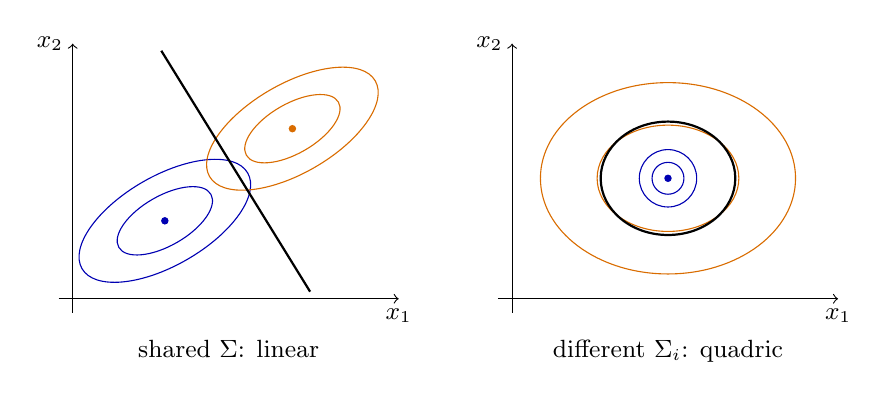
\begin{tikzpicture}[scale=0.9]
    \begin{scope}
      \draw[->] (-0.2,0) -- (4.6,0) node[below] {\small $x_1$};
      \draw[->] (0,-0.2) -- (0,3.6) node[left] {\small $x_2$};
      \foreach \s in {0.5,0.9} {
        \draw[blue!70!black, rotate around={30:(1.3,1.1)}]
          (1.3,1.1) ellipse ({1.5*\s} and {0.7*\s});
        \draw[orange!85!black, rotate around={30:(3.1,2.4)}]
          (3.1,2.4) ellipse ({1.5*\s} and {0.7*\s});
      }
      \fill[blue!70!black] (1.3,1.1) circle (1.5pt);
      \fill[orange!85!black] (3.1,2.4) circle (1.5pt);
      \draw[thick] (1.25,3.5) -- (3.35,0.1);
      \node[below] at (2.2,-0.45) {\small shared $\Sigma$: linear};
    \end{scope}
    \begin{scope}[xshift=6.2cm]
      \draw[->] (-0.2,0) -- (4.6,0) node[below] {\small $x_1$};
      \draw[->] (0,-0.2) -- (0,3.6) node[left] {\small $x_2$};
      \foreach \s in {0.5,0.9} {
        \draw[blue!70!black] (2.2,1.7) ellipse ({0.45*\s} and {0.45*\s});
        \draw[orange!85!black] (2.2,1.7) ellipse ({2.0*\s} and {1.5*\s});
      }
      \fill[blue!70!black] (2.2,1.7) circle (1.5pt);
      \draw[thick] (2.2,1.7) ellipse (0.95 and 0.8);
      \node[below] at (2.2,-0.45) {\small different $\Sigma_i$: quadric};
    \end{scope}
  \end{tikzpicture}
  \caption{Decision boundaries (black) for two Gaussian classes, drawn as
  contours of equal density. Left: with a shared covariance the quadratic terms
  cancel and the boundary is a straight line, tilted by $\Sigma^{-1}$. Right: a
  narrow class inside a wide one with the same mean gives a closed, elliptic
  boundary; the narrow class wins only near the center.}
  \label{fig:discr-cases}
\end{figure}

\noindent
Everything above assumes that the class-conditional densities are known. In
practice their shape is at best known in principle (for example ``Gaussian'')
while the parameters are not, and often considerably less is known. The rest of
the section is about estimating these densities from data, and about methods
that are as insensitive as possible to wrong assumptions.

\subsection{Non-Parametric Density Estimation}

A Bayes-optimal classifier is possible if the prior and the likelihood are
known. Priors are usually given or assumed uniform. Likelihoods must be
estimated from \emph{training data}: measurements for which the target value, for
example the class label, is known. The question the estimate answers is: how
often does a feature value occur given the class? There are two ways to answer
it. Non-parametric methods estimate the density directly from the samples, with
no assumption about its shape. Parametric methods assume a functional form with
a few parameters and fit those.

\paragraph{Histograms.}
The simplest estimate divides the feature range into bins and counts. The
probability of a bin is the fraction of samples that fall into it, a
frequentist interpretation of probability as the ratio of positive events to
possible events; dividing by the bin volume turns this into a density. The
estimate is \emph{consistent}: as the number of samples $\lvert D\rvert\to\infty$
(with suitably shrinking bins) it converges to the true distribution. Two
problems limit it. The bin width must be chosen: many narrow bins give a fine
resolution but need a lot of data, otherwise most bins are empty or noisy; few
wide bins are stable but blur the shape. And the number of cells explodes with
the dimension, the \emph{curse of dimensionality}: with $n$ bins per axis, $d$
dimensions need $n^d$ cells, so the number of samples required to fill them
grows exponentially. Ten bins in ten dimensions are already $10^{10}$ cells.
Empty bins produce zero probabilities, which a product of likelihoods cannot
recover from; the Laplace correction against this is covered in
Appendix~\ref{app:gmm}.

\paragraph{Parzen windows.}
A histogram fixes the bins in advance and asks which bin a sample falls into.
Parzen windows turn this around and center a window on the query point $x$
itself. Let the window be a hypercube of side length $h_n$ and volume
$V_n = h_n^d$, and let
\begin{equation}
  \varphi(u) =
  \begin{cases}
    1 & \lvert u_j\rvert\le 0.5 \quad (j = 1,\dots,d),\\
    0 & \text{otherwise}
  \end{cases}
\end{equation}
\noindent
be the unit-cube indicator. Then
$k_n = \sum_{i=1}^n \varphi\bigl(\frac{x-x_i}{h_n}\bigr)$ counts the samples
inside the window around $x$, and the density estimate is ``fraction of samples
per volume'':
\begin{equation}
  p_n(x) = \frac{k_n/n}{V_n}
  = \frac{1}{n}\sum_{i=1}^{n}\frac{1}{h_n^d}\,
    \varphi\Bigl(\frac{x-x_i}{h_n}\Bigr).
  \label{eq:parzen}
\end{equation}
\noindent
Read from the right, the formula says: put a small bump of volume one around
every sample and average the bumps. If the window function is itself a density,
$\varphi(u)\ge 0$ and $\int\varphi(u)\,du = 1$, then $p_n$ is a valid density.
The box is only one choice; a Gaussian window gives a smooth estimate
(Figure~\ref{fig:parzen}). The width $h_n$ plays the role of the bin width: too
small and the estimate is a spiky sum of isolated peaks, too large and all
structure is smoothed away. A one-dimensional example with the box window: the
samples are $\{1,\ 2,\ 2.5,\ 6\}$, $h = 2$, and we evaluate at $x = 2$. The window
covers $\lvert x-x_i\rvert\le 1$, which contains the three samples $1$, $2$ and
$2.5$, so $p(2) = 3/(4\cdot 2) = 0.375$.

\begin{figure}[ht]
  \centering
  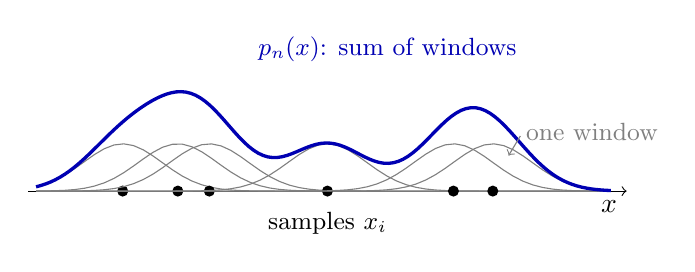
\begin{tikzpicture}[x=1cm, y=1cm]
    \draw[->] (-3.4,0) -- (4.2,0) node[below left] {$x$};
    \foreach \c in {-2.2,-1.5,-1.1,0.4,2.0,2.5} {
      \draw[gray, domain=-3.3:4, samples=60]
        plot (\x,{0.6*exp(-(\x-\c)^2/(2*0.25))});
      \fill (\c,0) circle (2pt);
    }
    \draw[very thick, blue!70!black, domain=-3.3:4, samples=120]
      plot (\x,{0.6*(exp(-(\x+2.2)^2/0.5)+exp(-(\x+1.5)^2/0.5)
        +exp(-(\x+1.1)^2/0.5)+exp(-(\x-0.4)^2/0.5)
        +exp(-(\x-2.0)^2/0.5)+exp(-(\x-2.5)^2/0.5))});
    \node[blue!70!black, right] at (-0.6,1.8) {\small $p_n(x)$: sum of windows};
    \node[gray, right] at (2.8,0.75) {\small one window};
    \draw[gray, ->] (2.85,0.7) -- (2.7,0.45);
    \node[below] at (0.4,-0.15) {\small samples $x_i$};
  \end{tikzpicture}
  \caption{Parzen window estimate with a Gaussian window. Each sample (dot)
  contributes one bump of width $h$ (gray); their average is the density
  estimate (blue, drawn unnormalized). Where samples cluster the bumps add up
  to a high density.}
  \label{fig:parzen}
\end{figure}

\paragraph{$k$-nearest-neighbor estimate.}
Parzen windows fix the volume and count the samples inside. The
$k$-nearest-neighbor (k-NN) estimate fixes the count instead: grow the window
around $x$ until it contains exactly $k$ samples, and use its volume $V_k(x)$,
\begin{equation}
  p(x) \approx \frac{k}{n\,V_k(x)} .
\end{equation}
\noindent
In dense regions the window stays small, in sparse regions it grows, so the
resolution adapts to the data. If the $k$ neighbors contain $k_i$ samples of
class $\omega_i$, the same reasoning gives the posterior estimate
$P(\omega_i\mid x)\approx k_i/k$, which is the k-NN classifier: vote among the
$k$ nearest training samples.

\subsection{Parametric Estimation}

Non-parametric methods are very general and make no assumption about the true
distribution, but they need a lot of data and must store all of it. Often the
general form of the density is known, or can be approximated well enough, and
can be parameterized, for example as a Gaussian. This reformulates a hopeless
problem, estimating the density at every point, into an easy one, estimating a
few numbers such as a mean and a variance. Table~\ref{tab:density-methods}
contrasts the families.

\begin{table}[ht]
  \centering
  \begin{tabular}{@{}lp{4.6cm}p{5.6cm}@{}}
    \toprule
    Method & Type & Key choice and weakness \\
    \midrule
    Histogram & non-parametric & bin width; curse of dimensionality, empty bins \\
    Parzen windows & non-parametric & window width $h$; stores all samples \\
    $k$-NN & non-parametric & $k$; estimate is not smooth \\
    Gaussian (ML) & parametric & assumed shape; wrong if data are multimodal \\
    Gaussian mixture & parametric & number of components $K$ \\
    \bottomrule
  \end{tabular}
  \caption{Density estimators. Parametric methods have a fixed functional form
  with a fixed number of parameters. A piecewise-constant model
  $P(4i\le x<4(i+1)) = \theta_i$ with its $25$ parameters $\theta_i$ is written
  in this parametric form, while histograms and Parzen windows are the standard
  non-parametric examples. Both Parzen windows and ML estimation yield a
  distribution over the data.}
  \label{tab:density-methods}
\end{table}

\paragraph{Maximum-likelihood estimation.}
Assume the class-conditional density has a known parametric form, for example
$p(x\mid\omega_j) = p(x\mid\omega_j,\theta_j)$ with
$\theta_j = (\mu_j,\Sigma_j)$ for a Gaussian. The training samples of each class
are used to estimate its unknown parameter vector. If the samples
$D = \{x_1,\dots,x_n\}$ are drawn independently, the probability of the whole
training set under the model $\theta$ is the product
\begin{equation}
  p(D\mid\theta) = \prod_{k=1}^{n} p(x_k\mid\theta),
  \qquad
  \hat\theta = \arg\max_\theta p(D\mid\theta).
  \label{eq:ml}
\end{equation}
\noindent
Viewed as a function of $\theta$, $p(D\mid\theta)$ is the \emph{likelihood of
the model}, and the ML estimate is the model that makes the observed data most
probable: the one that best explains them. In practice one maximizes the
\emph{log-likelihood} $\ell(\theta) = \sum_k \ln p(x_k\mid\theta)$, which has the
same maximum and turns the product into a sum, by setting its derivative to
zero. The recipe for every exercise of this kind is: write down $\ell(\theta)$,
differentiate, set to zero, solve.

For a Gaussian, $\ell(\mu) = \sum_k \bigl[-\frac12\ln(2\pi\sigma^2)
- \frac{(x_k-\mu)^2}{2\sigma^2}\bigr]$ and
$\partial\ell/\partial\mu = \sum_k (x_k-\mu)/\sigma^2 = 0$ gives the sample
mean. The same computation for the covariance gives the sample covariance:
\begin{equation}
  \hat\mu = \frac1n\sum_{k=1}^n x_k,
  \qquad
  \hat C = \frac{1}{n-1}\sum_{k=1}^n (x_k-\hat\mu)(x_k-\hat\mu)^\top .
  \label{eq:ml-gauss}
\end{equation}
\noindent
The exact ML solution divides by $n$; dividing by $n-1$ removes its small bias,
because $\hat\mu$ was fitted to the same data. The difference vanishes for large
$n$. With $n = 2$ samples the estimate is essentially arbitrary; with $10$,
$100$, and $1000$ samples the fitted Gaussian approaches the true one. A
million samples give a very precise estimate, but only of the assumed model: if
the data are not Gaussian (for example bimodal), more samples do not fix the
wrong shape.

The same recipe works for discrete models. For a count of errors per time
interval modeled as Poisson, $P(k) = \lambda^k e^{-\lambda}/k!$, with
measurements $X = \{2,3,8,6,4\}$:
\begin{equation}
  \ell(\lambda) = \sum_{i}\bigl[k_i\ln\lambda - \lambda - \ln k_i!\bigr],
  \qquad
  \frac{d\ell}{d\lambda} = \frac{\sum_i k_i}{\lambda} - n = 0
  \;\Rightarrow\;
  \hat\lambda = \frac1n\sum_i k_i = \frac{23}{5} = 4.60 .
\end{equation}
\noindent
For the day $k$ of the first production failure modeled as geometric,
$P(k) = (1-p)^{k-1}p$, with $D = \{8,6,10,9,4\}$:
\begin{equation}
  \ell(p) = \sum_i\bigl[(k_i-1)\ln(1-p) + \ln p\bigr],
  \qquad
  \frac{d\ell}{dp} = -\frac{\sum_i(k_i-1)}{1-p} + \frac{n}{p} = 0
  \;\Rightarrow\;
  \hat p = \frac{n}{\sum_i k_i} = \frac{5}{37}\approx 0.14 .
\end{equation}
\noindent
The step from the derivative to the result is
$n(1-p) = p\sum_i(k_i-1) = p\sum_i k_i - pn$, so $n = p\sum_i k_i$. The estimate
is one over the mean waiting time, which matches intuition: failures every
$7.4$ days on average mean a daily failure probability of about $1/7.4$. Always
insert the model exactly as stated; the formula for $\hat p$ changes if $k$ is
defined differently.

\paragraph{Bayesian estimation.}
ML treats the parameter as a fixed unknown number and picks one value. Bayesian
estimation treats the parameter itself as a random variable. Prior knowledge
enters in three forms: the shape of the unknown density $p(x\mid\theta)$, a
prior density $p(\theta)$ that expresses what is known about the parameter
values beforehand, and the training samples. The training data turn the prior
into a posterior with Bayes' theorem,
\begin{equation}
  p(\theta\mid D) = \frac{p(D\mid\theta)\,p(\theta)}{p(D)},
  \qquad
  p(x\mid D) = \int p(x\mid\theta)\,p(\theta\mid D)\,d\theta ,
  \label{eq:bayes-est}
\end{equation}
\noindent
and the density used for classification is the \emph{predictive} density
$p(x\mid D)$: an average over all models, each weighted by how well it is
supported by the data. The class posterior becomes
$P(\omega_i\mid x,D) = p(x\mid\omega_i,D)P(\omega_i)/\sum_j p(x\mid\omega_j,D)P(\omega_j)$.
The hope is that $p(\theta\mid D)$ has a sharp maximum at the true parameter
value. When it does, the integral is dominated by that single value and the
Bayesian result equals the ML (or MAP) plug-in estimate; this happens with many
training samples, and with a flat prior the peak lies exactly at the ML
estimate.

A discrete example shows the three strategies side by side. Two candidate
models $\theta_1$, $\theta_2$ have likelihoods $P(D\mid\theta_1) = 2\cdot10^{-6}$
and $P(D\mid\theta_2) = 10^{-6}$ on the data, priors $P(\theta_1) = 1/4$ and
$P(\theta_2) = 3/4$, and predict a new sample with
$P(x\mid\theta_1) = 1/4$, $P(x\mid\theta_2) = 1/3$.
\begin{itemize}
  \item ML selects the model with the larger likelihood, $\theta_1$, so
        $P(x\mid D) = 1/4$.
  \item MAP compares $P(D\mid\theta)P(\theta)$:
        $2\cdot10^{-6}\cdot\frac14 = 0.5\cdot10^{-6}$ against
        $10^{-6}\cdot\frac34 = 0.75\cdot10^{-6}$. It selects $\theta_2$, so
        $P(x\mid D) = 1/3$.
  \item Bayesian estimation normalizes these two numbers into the posteriors
        $P(\theta_1\mid D) = 0.5/1.25 = 0.4$ and $P(\theta_2\mid D) = 0.6$, and
        averages the predictions:
        $P(x\mid D) = 0.4\cdot\frac14 + 0.6\cdot\frac13 = 0.1 + 0.2 = 3/10$.
\end{itemize}
\noindent
The same normalization answers the plain posterior question: with
$P(D\mid\Omega_1) = 0.9$, $P(D\mid\Omega_2) = 0.43$ and priors $0.72$, $0.28$,
\begin{equation}
  P(\Omega_1\mid D) = \frac{0.9\cdot0.72}{0.9\cdot0.72 + 0.43\cdot0.28}
  = \frac{0.648}{0.7684}\approx 0.8433 .
\end{equation}
\noindent
Table~\ref{tab:ml-map-bayes} summarizes the differences. Instead of the density
function itself, all parametric methods search for its parameters.
When one Gaussian is too rigid, a mixture of several Gaussians fitted with
the EM algorithm is the usual parametric extension; it is summarized together
with probability calibration in Appendix~\ref{app:gmm}.

\begin{table}[ht]
  \centering
  \begin{tabular}{@{}lp{3.6cm}p{3.4cm}p{3.6cm}@{}}
    \toprule
    & ML & MAP & Bayesian \\
    \midrule
    Parameter is & fixed unknown & fixed unknown & random variable \\
    Maximizes & $p(D\mid\theta)$ & $p(D\mid\theta)\,p(\theta)$ &
      nothing; integrates over $\theta$ \\
    Result & one $\hat\theta$ & one $\hat\theta$ & posterior $p(\theta\mid D)$ \\
    Prediction & $p(x\mid\hat\theta)$ & $p(x\mid\hat\theta)$ &
      $\int p(x\mid\theta)p(\theta\mid D)\,d\theta$ \\
    Coincides with ML & --- & uniform prior & sharp posterior at $\hat\theta_{\mathrm{ML}}$ \\
    \bottomrule
  \end{tabular}
  \caption{Three ways of estimating parameters from training data $D$. ML
  explains the data, MAP adds prior knowledge, and Bayesian estimation keeps
  the full uncertainty about the parameters.}
  \label{tab:ml-map-bayes}
\end{table}

\subsection{Markov Random Fields}

So far the prior was one number per class, the same for every pixel. Images
contain much more prior knowledge than that. In the real world, dependencies
occur between neighboring objects, not between objects far apart: buildings are
parallel to the street next to them, pixels of one land-use class form larger
coherent areas, and road segments connect to long roads and networks. A noisy
pixel that looks like background in the middle of a road is probably road. A
\emph{Markov random field} (MRF) turns this kind of knowledge into a prior over
whole label images, and Bayes' theorem combines it with the noisy observations.

The name describes the model. A \emph{field} is a spatial (2D or 3D)
arrangement of variables. \emph{Random} means that every variable takes its
value randomly. In a general random field each variable may depend on all
others; in a \emph{Markov} random field a variable depends only on its
neighbors. Given the values of its neighbors, a variable is independent of the
rest of the field. The variables, called primitives, can be nodes of a general
graph (graph-based MRF, for example regions or objects) or the pixels of a
raster (raster-based MRF). Table~\ref{tab:mrf-terms} lists the vocabulary.

\begin{table}[ht]
  \centering
  \begin{tabular}{@{}lp{9.6cm}@{}}
    \toprule
    Term & Meaning \\
    \midrule
    Neighborhood relation & a line connecting two primitives \\
    Neighborhood of $s$ & all primitives with a neighborhood relation to $s$,
      written $\partial s$ \\
    Neighborhood system & set of all neighborhoods of the field, e.g.\ the
      4-neighborhood on a raster \\
    Clique & subset of primitives that are all neighbors of each other, e.g.\
      single pixels and horizontal or vertical pixel pairs \\
    Maximal clique & clique that cannot be enlarged by another primitive \\
    Potential $H_c$ & energy as a function of the states of the primitives of
      clique $c$; low energy means a likely configuration \\
    \bottomrule
  \end{tabular}
  \caption{Vocabulary of Markov random fields.}
  \label{tab:mrf-terms}
\end{table}

\paragraph{From potentials to probabilities.}
An MRF is specified by its potentials. The \emph{energy} of a complete
configuration $x$ is the sum of the potentials of all cliques $C$, and the
probability follows the Gibbs distribution:
\begin{equation}
  H(x) = \sum_{c\in C} H_c(x),
  \qquad
  p(x) = \frac1Z\exp\Bigl\{-\frac{H(x)}{T}\Bigr\},
  \qquad
  Z = \sum_{x\in\Omega}\exp\Bigl\{-\frac{H(x)}{T}\Bigr\}.
  \label{eq:gibbs}
\end{equation}
\noindent
Low energy means high probability, and a sum of energies becomes a product of
factors, one per clique. The temperature $T$ controls how peaked the
distribution is and is used in simulated annealing. The normalization constant
$Z$ sums over the whole configuration space $\Omega$, which for an image of
$N$ binary pixels has $2^N$ elements and cannot be computed. The Markov property
rescues us: the \emph{local} conditional probability of one primitive $s$ given
its neighbors involves only the cliques $C_s$ that contain $s$,
\begin{equation}
  H_s(x_s\mid x_{\partial s}) = \sum_{c\in C_s} H_c(x_s, x_{\partial s}),
  \qquad
  p(x_s\mid x_{\partial s})
  = \frac{1}{Z_s}\exp\Bigl\{-\frac{H_s(x_s\mid x_{\partial s})}{T}\Bigr\},
  \label{eq:local-gibbs}
\end{equation}
\noindent
where the local normalizer $Z_s$ sums only over the few states $\Lambda_s$ of
the single primitive $s$.

\paragraph{Example: horizontal lines.}
Suppose the world contains preferably horizontal one-pixel-wide lines, and line
interruptions and line ends are rare. The model uses the pixels as primitives
of a raster MRF, each with state $L$ (line, black) or $N$ (no line, white), the
4-neighborhood system, and horizontal and vertical two-pixel cliques. The
potentials in Figure~\ref{fig:mrf-potentials} make the unwanted configurations
expensive: a horizontal pair with one line and one non-line pixel, which is a
line end or an interruption, costs $\alpha$; a vertical pair of two line
pixels, which would make the line thicker than one pixel, costs $\beta$; every
other pair costs nothing.

\begin{figure}[ht]
  \centering
  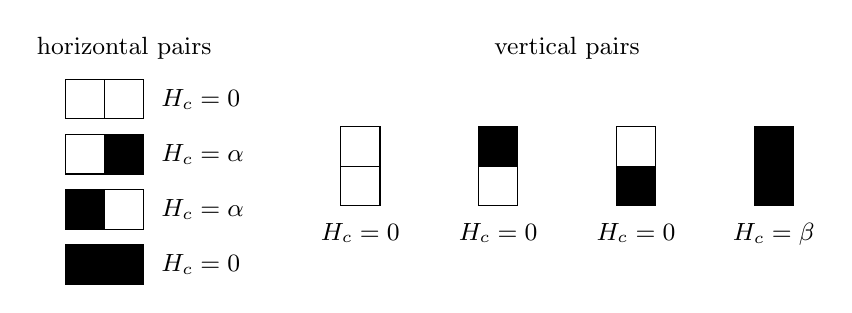
\begin{tikzpicture}[x=0.5cm, y=0.5cm]
    \tikzset{px/.style={draw, minimum size=0.5cm, inner sep=0pt},
             L/.style={px, fill=black}, N/.style={px, fill=white}}
    % horizontal cliques
    \node[font=\small] at (1,5.3) {horizontal pairs};
    \foreach \a/\b/\h [count=\i] in {N/N/0, N/L/\alpha, L/N/\alpha, L/L/0} {
      \node[\a] at (0,{5.4-1.4*\i}) {};
      \node[\b] at (1,{5.4-1.4*\i}) {};
      \node[right, font=\small] at (1.7,{5.4-1.4*\i}) {$H_c = \h$};
    }
    % vertical cliques
    \node[font=\small] at (12.25,5.3) {vertical pairs};
    \foreach \a/\b/\h/\xx in {N/N/0/7, L/N/0/10.5, N/L/0/14, L/L/\beta/17.5} {
      \node[\a] at (\xx,2.8) {};
      \node[\b] at (\xx,1.8) {};
      \node[below, font=\small] at (\xx,1.1) {$H_c = \h$};
    }
  \end{tikzpicture}
  \caption{Potentials of the two-pixel cliques for the horizontal-line model
  (black: line $L$, white: no line $N$), for example with $\alpha = \beta = 1$.
  Horizontal changes between $L$ and $N$ (line ends) and vertically stacked line
  pixels (thick lines) are penalized.}
  \label{fig:mrf-potentials}
\end{figure}

\noindent
The local conditional probability follows by adding the potentials of the four
cliques that contain the pixel $s$, once for each of its possible states. Take
$\alpha = \beta = T = 1$.
\begin{itemize}
  \item Left and right neighbors are $L$, top and bottom are $N$ (a gap in a
        line). If $s = N$, both horizontal pairs are $L$--$N$ changes, so
        $H_s(N) = 2\alpha = 2$; the vertical pairs cost nothing. If $s = L$, the
        horizontal pairs are $L$--$L$ and the vertical pairs have one $L$, so
        $H_s(L) = 0$. Hence
        $p(L\mid\partial s) = 1/(1+e^{-2})\approx 0.88$: the gap is probably
        filled.
  \item Only the top neighbor is $L$, the others are $N$. If $s = N$ nothing is
        penalized, $H_s(N) = 0$. If $s = L$, two horizontal changes and one
        vertical $L$--$L$ pair give $H_s(L) = 2\alpha + \beta = 3$, so
        $p(L\mid\partial s) = e^{-3}/(1+e^{-3})\approx 0.05$.
\end{itemize}

\paragraph{Estimating object parameters.}
The observations $y$ are the noisy grey values, and the object parameters to be
estimated are the hidden states $\varepsilon$ ($L$ or $N$) of all pixels. Bayes'
theorem $p(\varepsilon\mid y)\propto p(y\mid\varepsilon)\,p(\varepsilon)$ applies
locally, with the MRF as prior:
\begin{equation}
  p(\varepsilon_s\mid\varepsilon_{\partial s}, y_s)
  \propto p(y_s\mid\varepsilon_s)\;p(\varepsilon_s\mid\varepsilon_{\partial s}),
  \qquad
  p(y_s\mid\varepsilon_s)
  = \frac{1}{\sqrt{2\pi}\,\sigma_{\varepsilon}}
    \exp\Bigl\{-\frac{(y_s-\mu_{\varepsilon})^2}{2\sigma_{\varepsilon}^2}\Bigr\},
  \label{eq:mrf-posterior}
\end{equation}
\noindent
with, for example, $\mu_L = 90$, $\sigma_L = 10$ (lines are dark) and
$\mu_N = 110$, $\sigma_N = 10$. The ML estimate uses only the likelihood and
labels each pixel by its own grey value. The MAP estimate includes the MRF
prior. Taking the negative logarithm turns Equation~\eqref{eq:mrf-posterior}
into a sum of energies: a \emph{unary} (association) term
$(y_s-\mu_{\varepsilon_s})^2/(2\sigma^2)$ that ties each label to its own
observation, and \emph{pairwise} (interaction) terms $H_c/T$ that tie
neighboring labels together. This is the typical MRF of image processing: a
grid of hidden labels, each connected to its observation and to its four
neighbors. A worked pixel: $y_s = 105$ in the gap of case one above. Its unary
energies are $15^2/200 = 1.125$ for $L$ and $5^2/200 = 0.125$ for $N$, so ML says
$N$. Adding the prior energies $0$ and $2$ gives $1.125$ for $L$ against
$2.125$ for $N$, so MAP says $L$ and closes the gap.

Because every label depends on its neighbors, which are themselves being
estimated, the MAP configuration is found iteratively. Simulated annealing
visits the pixels repeatedly, draws each new state from its local posterior at
temperature $T$, and lowers the temperature slowly, for example as
$T_i = 0.7/\ln(i)$ over the iterations $i$. At high temperature the states
change freely and the search can escape poor configurations; as $T\to 0$ the
local posteriors become deterministic and the field freezes into a
low-energy, high-posterior labeling. On noisy observations of horizontal
lines, the ML result is a scatter of isolated line pixels and holes, while the
MAP result recovers mostly continuous horizontal lines with few defects.

\paragraph{Estimating model parameters.}
The prior parameters $\alpha$ and $\beta$ need not be guessed. Given training
images with known ``true'' object parameters, the model can be adapted to a
dataset: run the MAP estimation with the current parameters, measure the
difference between estimate and truth, and let this evaluation control a
simulated annealing search over the parameters themselves. In the line
example, optimizing the parameters from $\alpha = \beta = 1.0$ to
$\alpha = 2.2$, $\beta = 1.0$ penalizes interruptions more strongly and yields
visibly cleaner lines. Conditional random fields, which condition the pairwise
terms on the observations, and the factorization rules of graphical models in
general are summarized in Appendix~\ref{app:graphical}.

The whole section rests on one principle. The best decision minimizes the
expected risk, and for the error probability this means choosing the class of
maximum posterior. The difficulty is almost never the decision rule but the
probabilities it needs: likelihoods have to be estimated from limited data,
either freely or through a parametric model, and priors, from class
frequencies up to Markov random fields, supply the knowledge that the data
alone cannot.
